\documentclass[11pt]{article}

\usepackage[margin=1in]{geometry}
\usepackage[T1]{fontenc}
\usepackage{lmodern}
\usepackage{microtype}
\usepackage{amsmath,amssymb,amsthm,mathtools}
\usepackage{mathrsfs}
\usepackage[dvipsnames]{xcolor}
\usepackage[most]{tcolorbox}
\usepackage{tikz}
\usetikzlibrary{decorations.markings,patterns}
\usepackage{enumitem}
\usepackage{tocloft}
\usepackage[hidelinks]{hyperref}

\definecolor{courseblue}{HTML}{1F4E79}
\definecolor{lightblue}{HTML}{EAF2F8}
\definecolor{lightgreen}{HTML}{EAF7EA}
\definecolor{lightpink}{HTML}{FCE8EF}
\definecolor{lightyellow}{HTML}{FFF8D6}
\definecolor{warningyellow}{HTML}{D6A000}
\definecolor{exercisebg}{HTML}{FDEAEA}
\definecolor{exerciseframe}{HTML}{B54040}
\definecolor{examplebg}{HTML}{F4FAFE}
\definecolor{exampleframe}{HTML}{85C1E9}
\definecolor{darkgray}{HTML}{333333}
\definecolor{lightorange}{HTML}{FDEBD8}
\definecolor{orangeframe}{HTML}{E08A3C}

\setlength{\parindent}{0pt}
\setlength{\parskip}{0.65em}
\setlist[itemize]{topsep=0.25em,itemsep=0.15em}
\renewcommand{\cftsecleader}{\cftdotfill{\cftdotsep}}
\renewcommand{\cftsubsecleader}{\cftdotfill{\cftdotsep}}

\theoremstyle{plain}
\newtheorem{theorem}{Theorem}[section]
\newtheorem{proposition}[theorem]{Proposition}
\newtheorem{lemma}[theorem]{Lemma}
\newtheorem{corollary}[theorem]{Corollary}
\theoremstyle{definition}
\newtheorem{definition}[theorem]{Definition}
\newtheorem{example}[theorem]{Example}
\newtheorem{exercise}[theorem]{Exercise}
\theoremstyle{remark}
\newtheorem*{remark}{Remark}
\newtheorem*{fact}{Fact}
\newtheorem*{warning}{Warning}

\tcolorboxenvironment{definition}{
  enhanced,
  unbreakable,
  colback=lightgreen,
  colframe=ForestGreen,
  boxrule=0.7pt,
  arc=2pt,
  left=6pt,
  right=6pt,
  top=5pt,
  bottom=5pt
}

\tcolorboxenvironment{warning}{
  enhanced,
  colback=lightyellow,
  colframe=warningyellow,
  boxrule=0.7pt,
  arc=2pt,
  left=6pt,
  right=6pt,
  top=5pt,
  bottom=5pt
}

\tcolorboxenvironment{exercise}{
  enhanced,
  colback=exercisebg,
  colframe=exerciseframe,
  boxrule=1pt,
  arc=2pt,
  left=6pt,
  right=6pt,
  top=5pt,
  bottom=5pt
}

\tcolorboxenvironment{example}{
  enhanced,
  colback=examplebg,
  colframe=exampleframe,
  boxrule=0.7pt,
  arc=2pt,
  left=6pt,
  right=6pt,
  top=5pt,
  bottom=5pt
}

\numberwithin{equation}{section}

\newcommand{\be}{\begin{eqnarray}}
\newcommand{\ee}{\end{eqnarray}}
\newcommand{\C}{\mathbb{C}}
\newcommand{\R}{\mathbb{R}}
\newcommand{\N}{\mathbb{N}}
\newcommand{\Z}{\mathbb{Z}}
\DeclareMathOperator{\Log}{Log}
\DeclareMathOperator{\Arg}{Arg}

\DeclareMathOperator{\Hol}{\mathcal{H}\mathrm{ol}}
\DeclareMathOperator{\Real}{Re}
\DeclareMathOperator{\Imag}{Im}
\newcommand{\A}{\mathcal{A}}
\newcommand{\CT}{\C[[T]]}
\newcommand{\CLT}{\C((T))}
\tcbset{breakable}
\begin{document}

\begin{center}
  \colorbox{lightblue}{%
    \begin{minipage}{0.94\textwidth}
      \vspace{0.55em}
      \begin{tabular*}{\textwidth}{@{\extracolsep{\fill}}lr}
        {\color{courseblue}\bfseries\LARGE Lecture 18} &
        {\color{courseblue}\bfseries\LARGE MATH 411}\\[0.35em]
        \textbf{Fall 2026} & \textbf{Date: Oct 21, 2026}\\
        & \textbf{Instructor: Manish Patnaik}
      \end{tabular*}
      \vspace{0.45em}
    \end{minipage}}
\end{center}

\setcounter{tocdepth}{1}
\tableofcontents
\vspace{0.45em}


% Sources: current Lectures 16 and 17; handwritten Lecture 18, Oct. 24,
% pages 1--6. The circle comparison is moved from the end of Lecture 17.
% The handwritten order and geometric sketches are preserved; details are
% supplied for path independence, local differentiation, and logarithm branches.
We review the homotopy form of Cauchy's theorem, recall the local Cauchy
integral formula, and justify the comparison of circles used in its proof.
We then continue with global primitives and complex logarithms.
Throughout, homotopies have \emph{fixed endpoints}, as in Lecture~17.

\section{Review: the homotopy form of Cauchy's theorem}
\begin{theorem}[Homotopy form of Cauchy's theorem]\label{thm:homotopy}
Let $U\subseteq\C$ be open and $f$ holomorphic on $U$.
If continuous curves $\gamma,\eta\colon[a,b]\to U$ are homotopic
with fixed endpoints in $U$, then
\[
 \boxed{\displaystyle\int_\gamma f(z)\,dz=\int_\eta f(z)\,dz.}
\]
\end{theorem}
Recall that the homotopy is a continuous map
$H\colon[a,b]\times[0,1]\to U$ with
\[
 H(t,0)=\gamma(t),\quad H(t,1)=\eta(t),\quad
 H(a,s)=\gamma(a),\quad H(b,s)=\gamma(b).
\]
The last two equalities hold for every $s\in[0,1]$.

\begin{center}
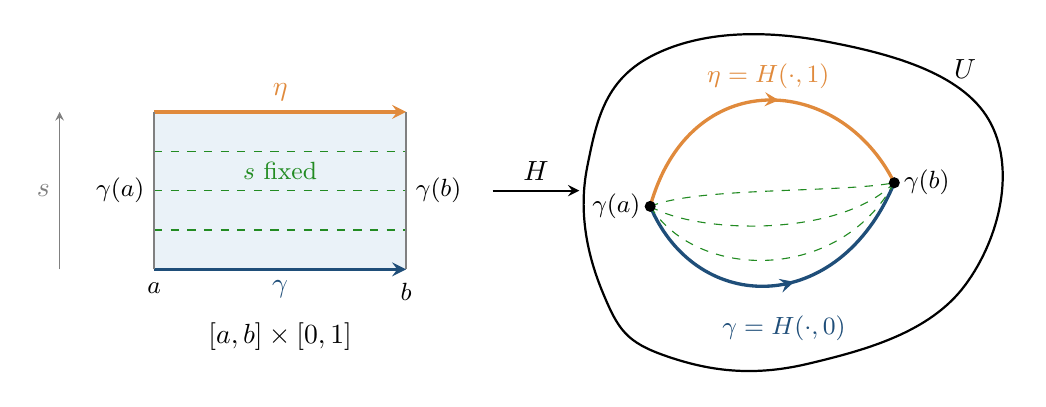
\begin{tikzpicture}[>=stealth,
 decoration={markings,mark=at position 0.55 with {\arrow{>}}}]
 % parameter rectangle
 \fill[lightblue] (0,0) rectangle (3.2,2);
 \foreach \y in {0.5,1,1.5}
  \draw[ForestGreen,thin,dashed] (0,\y)--(3.2,\y);
 \draw[courseblue,very thick,->] (0,0)--(3.2,0) node[midway,below]{$\gamma$};
 \draw[orangeframe,very thick,->] (0,2)--(3.2,2) node[midway,above]{$\eta$};
 \draw[gray,thick] (0,0)--(0,2) (3.2,0)--(3.2,2);
 \node[left,font=\small] at (0,1){$\gamma(a)$};
 \node[right,font=\small] at (3.2,1){$\gamma(b)$};
 \node[below,font=\small] at (0,-0.05){$a$};
 \node[below,font=\small] at (3.2,-0.05){$b$};
 \node[ForestGreen,font=\small] at (1.6,1.25){$s$ fixed};
 \draw[gray,->] (-1.2,0)--(-1.2,2) node[midway,left]{$s$};
 \node at (1.6,-0.85){$[a,b]\times[0,1]$};
 % arrow H
 \draw[->,thick] (4.3,1)--(5.4,1) node[midway,above]{$H$};
 % image in U
 \begin{scope}[xshift=5.9cm,yshift=-0.3cm]
  \draw[thick] plot[smooth cycle,tension=0.7] coordinates
  {(-0.2,0.0) (0.6,-0.8) (2.4,-0.9) (4.4,0.1) (4.7,2.2) (2.6,3.2) (0.4,3.0) (-0.4,1.6)};
  \node at (4.4,2.85){$U$};
  \draw[courseblue,very thick,postaction={decorate}] (0.4,1.1)
   .. controls (1,-0.3) and (2.8,-0.3) .. (3.5,1.4);
  \draw[orangeframe,very thick,postaction={decorate}] (0.4,1.1)
   .. controls (0.9,2.9) and (2.8,2.8) .. (3.5,1.4);
  \foreach \k in {0.45,1.05,1.65}
   \draw[ForestGreen,thin,dashed] (0.4,1.1)
    .. controls (1,-0.3+\k) and (2.8,-0.3+0.95*\k) .. (3.5,1.4);
  \fill (0.4,1.1) circle (2pt) node[left,font=\small]{$\gamma(a)$};
  \fill (3.5,1.4) circle (2pt) node[right,font=\small]{$\gamma(b)$};
  \node[courseblue,font=\small] at (2.1,-0.45){$\gamma=H(\cdot,0)$};
  \node[orangeframe,font=\small] at (1.9,2.75){$\eta=H(\cdot,1)$};
 \end{scope}
\end{tikzpicture}
\end{center}
Each horizontal line $s=\text{const.}$ in the rectangle is mapped to an
intermediate curve $H(\cdot,s)$ from $\gamma(a)$ to $\gamma(b)$; the
vertical edges are collapsed to the two endpoints.
The proof in Lecture~17 used local primitives to compare curves in a
common chain of discs, then compactness and uniform continuity to split
a homotopy into finitely many such comparisons.

\begin{definition}  A subset $U \subset \C$ is said to be \emph{simply connected} if $U$ is nonempty, open,	connected, and every closed continuous curve in $U$ is null-homotopic, i.e. the curve is homotopic to the constant curve. \end{definition}

\begin{corollary}\label{cor:null}
If $\gamma$ is null-homotopic in $U$, then $\int_\gamma f(z)\,dz=0$.
In particular, this holds for every closed continuous curve when $U$ is
simply connected.
\end{corollary}
\begin{proof}
A null-homotopic curve can be deformed, with its base point fixed, to a
constant curve. The theorem preserves the integral, and a constant
curve has integral zero.
\end{proof}


\section{The local Cauchy integral formula}
\begin{theorem}[Local Cauchy integral formula]\label{thm:cauchy-formula}
Let $D=D(c,R)$, let $U$ be an open set containing $\overline D$, and
let $f$ be holomorphic on $U$. If $z_0\in D$ and
$\gamma(t)=c+Re^{it}$, $0\leq t\leq2\pi$, then
\[
 \boxed{\displaystyle f(z_0)=\frac{1}{2\pi i}
 \int_\gamma\frac{f(z)}{z-z_0}\,dz.}
\]
\end{theorem}

The proof in Lecture~16 hinged on a comparison of integrals over
different circles. Fix $0<r<R-|z_0-c|$ and let $C_r(t)=z_0+re^{it}$,
$0\leq t\leq2\pi$. The outer circle $\gamma$ has basepoint $p=c+R$ and
the inner circle $C_r$ has basepoint $q=z_0+r$. We would like to
establish that for every function $h$ holomorphic on $U\setminus\{z_0\}$,
\begin{equation}\label{eq:circle-comparison}
 \int_\gamma h(z)\,dz=\int_{C_r}h(z)\,dz.
\end{equation}
The issue is that the two curves are not homotopic in our sense, since
our homotopies have fixed endpoints and $p\neq q$.

To fix this issue, we consider the straight segment $\alpha$ from
$p$ to $q$:
\[
 \alpha(s)=(1-s)p+sq,\qquad 0\leq s\leq1.
\]


\begin{center}
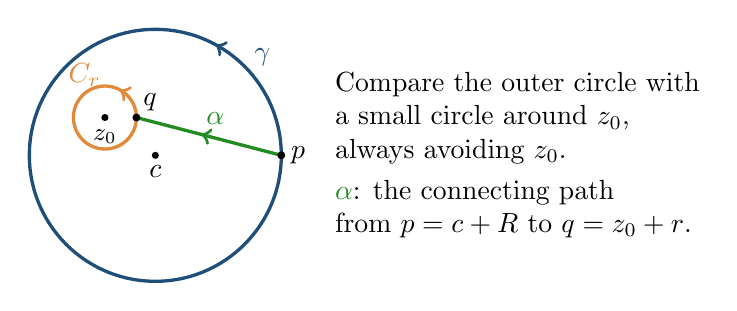
\begin{tikzpicture}[scale=0.8,
 decoration={markings,mark=at position 0.17 with {\arrow{>}}}]
 \draw[courseblue,very thick,postaction={decorate}] (2,0)
 arc[start angle=0,end angle=360,radius=2];
 \fill (0,0) circle (1.6pt) node[below]{$c$};
 \fill (-0.8,0.6) circle (1.6pt) node[below=1pt,font=\small]{$z_0$};
 \draw[orangeframe,very thick,postaction={decorate}] (-0.3,0.6)
 arc[start angle=0,end angle=360,radius=0.5];
 \draw[ForestGreen,very thick,
  decoration={markings,reset marks,mark=at position 0.55 with {\arrow{>}}},
  postaction={decorate}] (2,0)--(-0.3,0.6);
 \fill (2,0) circle (1.8pt) node[right]{$p$};
 \fill (-0.3,0.6) circle (1.8pt) node[above right=-1pt]{$q$};
 \node[ForestGreen] at (0.95,0.58){$\alpha$};
 \node[courseblue] at (1.7,1.55){$\gamma$};
 \node[orangeframe] at (-1.12,1.28){$C_r$};
 \node[right,align=left] at (2.7,0)
 {Compare the outer circle with\\a small circle around $z_0$,\\always avoiding $z_0$.\\[0.3em]
 {\color{ForestGreen}$\alpha$}: the connecting path\\from $p=c+R$ to $q=z_0+r$.};
\end{tikzpicture}
\end{center}


Write $\gamma*\alpha$ and $\alpha*C_r$ for the concatenated curves:
$\gamma*\alpha$ first follows $\gamma$ and then $\alpha$, and similarly
for $\alpha*C_r$. (Each piece is assigned half of the parameter
interval.) These two new curves have the advantage that they both begin
at $p$ and end at $q$. Moreover, there is a fixed-endpoint homotopy
between them in $U\setminus\{z_0\}$!


Consider the continuous map
\[
 F(t,s)=(1-s)c+sz_0+\bigl((1-s)R+sr\bigr)e^{it},
 \qquad 0\leq t\leq2\pi,\quad 0\leq s\leq1.
\]

Put $d=|z_0-c|<R$. The estimates
\begin{align*}
 |F(t,s)-c|&\leq sd+(1-s)R+sr\leq R,\\
 |F(t,s)-z_0|&\geq(1-s)(R-d)+sr>0
\end{align*}
show that $F$ takes values in $\overline D\setminus\{z_0\}$,
hence in $U\setminus\{z_0\}$. Its bottom and top edges give
$\gamma$ and $C_r$, and both vertical edges give the connecting path:
$F(0,s)=F(2\pi,s)=\alpha(s)$.



\begin{center}
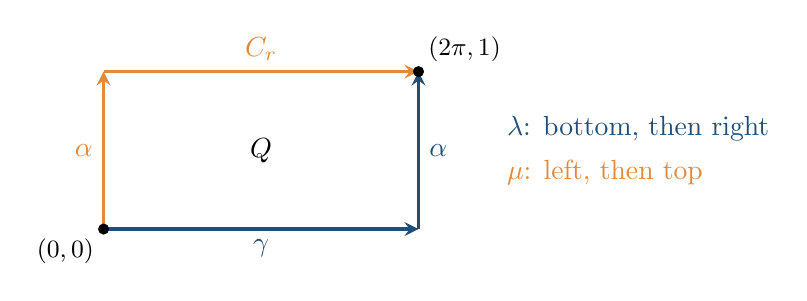
\begin{tikzpicture}[x=1cm,y=1cm,>=stealth]
 \draw[courseblue,very thick,->] (0,0)--(4,0)
  node[midway,below]{$\gamma$};
 \draw[courseblue,very thick,->] (4,0)--(4,2)
  node[midway,right]{$\alpha$};
 \draw[orangeframe,very thick,->] (0,0)--(0,2)
  node[midway,left]{$\alpha$};
 \draw[orangeframe,very thick,->] (0,2)--(4,2)
  node[midway,above]{$C_r$};
 \fill (0,0) circle (2pt);
 \fill (4,2) circle (2pt);
 \node[below left,font=\small] at (0,0){$(0,0)$};
 \node[above right,font=\small] at (4,2){$(2\pi,1)$};
 \node at (2,1){$Q$};
 \node[right,align=left] at (5,1)
  {{\color{courseblue}$\lambda$: bottom, then right}\\[0.4em]
   {\color{orangeframe}$\mu$: left, then top}};
\end{tikzpicture}
\end{center}


Let $Q=[0,2\pi]\times[0,1]$, and write
$\lambda,\mu\colon[0,1]\to Q$ for the two boundary paths shown above,
with each edge traversed linearly in half the parameter interval.
The path $\lambda$ follows the bottom and right edges; $\mu$ follows
the left and top edges. The labels in the picture are the images of
the edges under $F$, so
\[
 F\circ\lambda=\gamma*\alpha,\qquad F\circ\mu=\alpha*C_r.
\]

Both paths start at $(0,0)$ and end at $(2\pi,1)$. Since $Q$ is convex,
$\lambda$ and $\mu$ are homotopic in $Q$ with fixed endpoints, e.g.\ by
the straight-line homotopy
\[
 H(t,s)=(1-s)\lambda(t)+s\mu(t),\qquad 0\leq t,s\leq1.
\]
Composing $H$ with $F$ gives a continuous map
$[0,1]\times[0,1]\xrightarrow{H}Q\xrightarrow{F}U\setminus\{z_0\}$,
namely
\[
 C(t,s)=F\bigl((1-s)\lambda(t)+s\mu(t)\bigr),
 \qquad 0\leq t,s\leq1.
\]
This is a homotopy between $F\circ\lambda=\gamma*\alpha$ and
$F\circ\mu=\alpha*C_r$ in $U\setminus\{z_0\}$, with
$C(0,s)=p$ and $C(1,s)=q$ for every $s$.
Thus Theorem~\ref{thm:homotopy}, applied on the open set
$U\setminus\{z_0\}$, and additivity of integrals give
\[
 \int_\gamma h(z)\,dz+\int_\alpha h(z)\,dz
 =\int_\alpha h(z)\,dz+\int_{C_r}h(z)\,dz
 \qquad\bigl(h\in\Hol(U\setminus\{z_0\})\bigr).
\]
Cancelling the connecting-path integrals yields
\eqref{eq:circle-comparison}:
\[
 \int_\gamma h(z)\,dz=\int_{C_r}h(z)\,dz
 \qquad\text{for every }h\in\Hol(U\setminus\{z_0\}).
\]
Applying this to $h(z)=(f(z)-f(z_0))/(z-z_0)$ and to $h(z)=1/(z-z_0)$
justifies both circle comparisons in the proof from Lecture~16, and so
completes the proof of Theorem~\ref{thm:cauchy-formula}.
%
%Apply this to $h(z)=(f(z)-f(z_0))/(z-z_0)$ and $h(z)=1/(z-z_0)$.
%This justifies both comparisons in the preceding proof and completes it.
%
%The same argument compares the concentric circles in the punctured-disc
%example: use $F(t,s)=((1-s)r+s\rho)e^{it}$ and the connecting segment
%$\alpha(s)=(1-s)r+s\rho$. It gives
%$C_r*\alpha\sim\alpha*C_\rho$ with fixed endpoints, and hence
%equal integrals for every function holomorphic on the punctured disc.
%

\section{Primitives on simply connected domains}
% Handwritten Lecture 18, pages 1--3.
We know that a holomorphic function has a primitive on each \textit{disc} (this was a consequence of Cauchy--Goursat, proven for rectangles in discs).
The homotopy theorem now lets us replace the disc by any simply connected domain.

\begin{theorem}\label{thm:global-primitive}
Let $U\subseteq\C$ be simply connected and let $f$ be holomorphic on
$U$. Then $f$ has a primitive on all of $U$.
More precisely, fix $z_0\in U$ and define
\[
 g(z)=\int_{z_0}^z f(\zeta)\,d\zeta,
\]
where the integral is taken along any continuous curve in $U$ from
$z_0$ to $z$. This is well-defined, and $g'=f$ on $U$.
\end{theorem}

\begin{center}
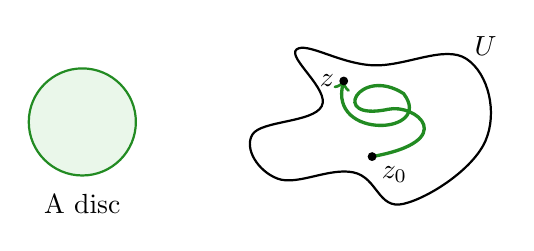
\begin{tikzpicture}[scale=0.8]
 \fill[lightgreen] (-2,0) circle (0.85);
 \draw[ForestGreen,thick] (-2,0) circle (0.85);
 \node[below] at (-2,-1){A disc};
 \begin{scope}[xshift=2.6cm]
  \draw[thick] plot[smooth cycle,tension=0.7] coordinates
  {(-1.5,-0.9) (-1.9,-0.2) (-0.8,0.25) (-1.2,1.15)
   (0,0.9) (1.5,1) (1.8,-0.3) (0.5,-1.3) (-0.3,-0.8)};
  \draw[ForestGreen,very thick,->] (0,-0.55)
   .. controls (1.4,-0.3) and (0.7,0.3) .. (0.25,0.2)
   .. controls (-0.7,0) and (-0.2,0.9) .. (0.5,0.45)
   .. controls (1,-0.2) and (-0.7,-0.3) .. (-0.45,0.65);
  \fill (0,-0.55) circle (2pt) node[below right]{$z_0$};
  \fill (-0.45,0.65) circle (2pt) node[left]{$z$};
  \node at (1.8,1.2){$U$};
 \end{scope}
\end{tikzpicture}
\end{center}

\begin{proof}
\textbf{Existence of paths.} A connected open subset of $\C$ is
polygonally connected.\footnote{An open set $U\subseteq\C$ is
\emph{polygonally connected} if any two points $z,w\in U$ can be joined
by a \emph{polygonal path} in $U$: a finite chain of line segments
$[w_0,w_1],[w_1,w_2],\dots,[w_{n-1},w_n]$, each contained in $U$, with
$w_0=z$ and $w_n=w$. A polygonal path is piecewise $C^1$, so in
particular it is a continuous curve along which we can integrate.}
To recall why, let $A$ consist of points reachable
from $z_0$ by a polygonal path in $U$. A small disc about any point of
$U$ lies in $U$. Joining points within this disc by segments shows that
both $A$ and $U\setminus A$ are open relative to $U$. Since $z_0\in A$
and $U$ is connected, $A=U$.

\textbf{Independence of the path.} Suppose $\gamma$ and $\eta$ both
run from $z_0$ to $z$ in $U$. Write $\eta^{-1}$ for $\eta$ traversed
backwards. Then $\gamma*\eta^{-1}$ is a closed curve in $U$.
It is null-homotopic because $U$ is simply connected, so
Corollary~\ref{cor:null} gives
\[
 0=\int_{\gamma*\eta^{-1}}f(\zeta)\,d\zeta
 =\int_\gamma f(\zeta)\,d\zeta-\int_\eta f(\zeta)\,d\zeta.
\]
Thus the definition of $g(z)$ does not depend on the chosen curve.

\begin{center}
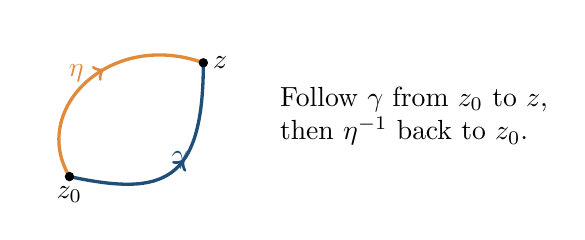
\begin{tikzpicture}[scale=0.85,
 decoration={markings,mark=at position 0.55 with {\arrow{>}}}]
 \draw[courseblue,very thick,postaction={decorate}] (0,0)
 .. controls (1.4,-0.3) and (2,-0.1) .. (2,1.7);
 \draw[orangeframe,very thick,postaction={decorate}] (0,0)
 .. controls (-0.6,1) and (0.6,2.2) .. (2,1.7);
 \fill (0,0) circle (2pt) node[below]{$z_0$};
 \fill (2,1.7) circle (2pt) node[right]{$z$};
 \node[courseblue] at (1.65,0.25){$\gamma$};
 \node[orangeframe] at (0.1,1.55){$\eta$};
 \node[right,align=left] at (3,0.9)
 {Follow $\gamma$ from $z_0$ to $z$,\\then $\eta^{-1}$ back to $z_0$.};
\end{tikzpicture}
\end{center}

\textbf{Differentiating locally.} Fix $z_1\in U$ and choose a disc
$B=D(z_1,\varepsilon)\subseteq U$. Let $G$ be a primitive of $f$ on
$B$. For $z\in B$, use a fixed path from $z_0$ to $z_1$ followed by
the straight segment from $z_1$ to $z$. Path independence gives
\[
 g(z)=g(z_1)+\int_{[z_1,z]}f(\zeta)\,d\zeta
     =g(z_1)+G(z)-G(z_1).
\]
\begin{center}
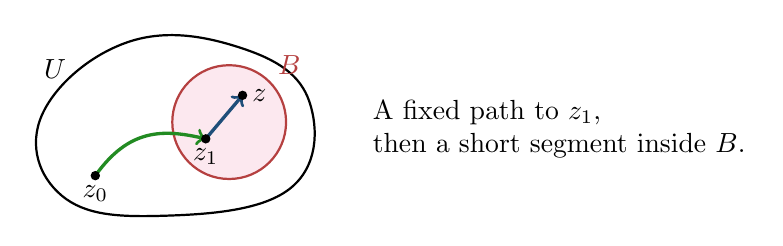
\begin{tikzpicture}[scale=0.85]
 \draw[thick] plot[smooth cycle,tension=0.7] coordinates
 {(-0.5,-0.7) (-0.8,0.5) (0.5,1.6) (2.2,1.5) (3.2,0.7) (2.9,-0.6) (1,-1)};
 \fill[lightpink] (2,0.4) circle (0.85);
 \draw[exerciseframe,thick] (2,0.4) circle (0.85);
 \draw[ForestGreen,very thick,->] (0,-0.4)
 .. controls (0.5,0.3) and (1,0.3) .. (1.65,0.15);
 \draw[courseblue,very thick,->] (1.65,0.15)--(2.2,0.8);
 \fill (0,-0.4) circle (2pt) node[below]{$z_0$};
 \fill (1.65,0.15) circle (2pt) node[below]{$z_1$};
 \fill (2.2,0.8) circle (2pt) node[right]{$z$};
 \node[exerciseframe] at (2.9,1.25){$B$};
 \node at (-0.6,1.2){$U$};
 \node[right,align=left] at (4,0.3)
 {A fixed path to $z_1$,\\then a short segment inside $B$.};
\end{tikzpicture}
\end{center}
The two terms involving $z_1$ are constant as $z$ varies in $B$.
Consequently $g'(z)=G'(z)=f(z)$ on $B$. Since $z_1$ was arbitrary,
$g$ is a primitive on all of $U$.
\end{proof}

\section{Complex logarithms}
% Handwritten Lecture 18, pages 3--6.
Recall that
\[
 e^w=\sum_{n=0}^\infty\frac{w^n}{n!},\qquad
 e^{x+iy}=e^x(\cos y+i\sin y).
\]
The exponential is never zero and has period $2\pi i$. We would like to
invert it. If $z=re^{i\theta}\ne0$, then all solutions of $e^w=z$ are
\[
 w=\ln r+i(\theta+2\pi k),\qquad k\in\Z.
\]
Here $\ln$ denotes the ordinary real logarithm. The difficulty is to
choose the argument continuously as $z$ varies.

\subsection{Why a branch is needed}
If we always choose $\theta\in[0,2\pi)$, the function
$\ln|z|+i\theta$ jumps across the positive real axis. At a positive
real number $r$, the limits from above and below are respectively
$\ln r$ and $\ln r+2\pi i$.

\begin{center}
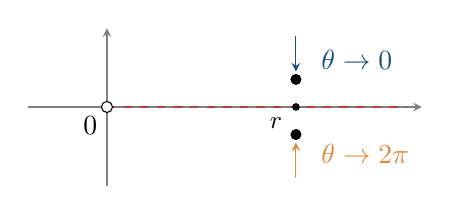
\begin{tikzpicture}[x=1cm,y=1cm,>=stealth]
 \draw[gray,->] (-1,0)--(4,0);
 \draw[gray,->] (0,-1)--(0,1);
 \draw[exerciseframe,dashed,thick] (0,0)--(3.8,0);
 \draw[fill=white] (0,0) circle (2pt) node[below left]{$0$};
 \fill (2.4,0.35) circle (2pt);
 \fill (2.4,-0.35) circle (2pt);
 \draw[courseblue,->] (2.4,0.9)--(2.4,0.45);
 \draw[orangeframe,->] (2.4,-0.9)--(2.4,-0.45);
 \node[right,courseblue] at (2.6,0.6){$\theta\to0$};
 \node[right,orangeframe] at (2.6,-0.6){$\theta\to2\pi$};
 \fill (2.4,0) circle (1.4pt);
 \node[left,font=\small] at (2.35,-0.2){$r$};
\end{tikzpicture}
\end{center}

In fact, no continuous function $L$ on $\C\setminus\{0\}$ satisfies
$e^{L(z)}=z$ for all $z\ne0$. If $L$ were one, then
\[
 L(e^{it})-it\in2\pi i\Z\qquad(0\leq t\leq2\pi).
\]
This continuous function of $t$ takes values in a discrete set, so it
is constant. But its values at $0$ and $2\pi$ differ by $-2\pi i$,
since $e^0=e^{2\pi i}=1$. This is a contradiction.

\begin{definition}
A \emph{holomorphic branch of the logarithm} on an open set
$U\subseteq\C\setminus\{0\}$ is a holomorphic function $L\colon U\to\C$
satisfying $e^{L(z)}=z$ for every $z\in U$.
\end{definition}
Differentiating this identity gives $e^{L(z)}L'(z)=1$, hence
$L'(z)=1/z$. This suggests constructing a logarithm by integrating $1/z$.

\subsection{Constructing a logarithm on a simply connected domain}
\begin{theorem}\label{thm:log-z}
Let $U\subseteq\C\setminus\{0\}$ be simply connected. Choose $z_0\in U$
and $w_0\in\C$ with $e^{w_0}=z_0$. Then
\[
 \boxed{\displaystyle L(z)=w_0+\int_{z_0}^z\frac{d\zeta}{\zeta}}
\]
defines a holomorphic branch of the logarithm on $U$, with
$L(z_0)=w_0$ and $L'(z)=1/z$.
\end{theorem}
\begin{proof}
The function $1/z$ is holomorphic on $U$, so Theorem~\ref{thm:global-primitive}
shows that the integral is path independent and $L'=1/z$.
To verify the exponential identity, differentiate:
\[
 \frac{d}{dz}\bigl(ze^{-L(z)}\bigr)
 =e^{-L(z)}-ze^{-L(z)}L'(z)=0.
\]
Since $U$ is connected, $ze^{-L(z)}$ is constant. At $z=z_0$ it equals
$z_0e^{-w_0}=1$, so $e^{L(z)}=z$ throughout $U$.
\end{proof}

\begin{center}
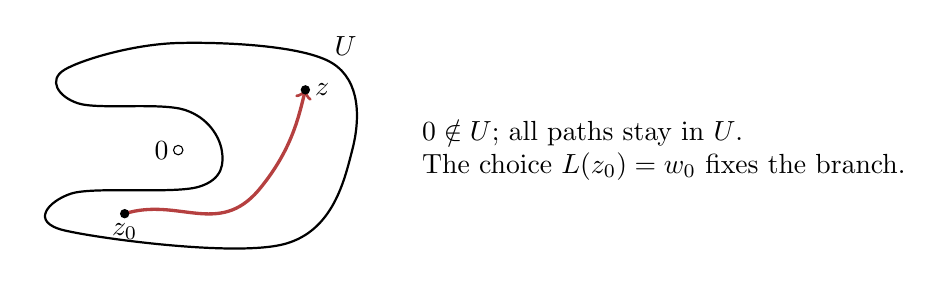
\begin{tikzpicture}[scale=0.85]
 \draw[thick] plot[smooth cycle,tension=0.6] coordinates
 {(-1.7,1.2) (0,1.6) (2.3,1.3) (2.6,0) (1.6,-1.4)
  (-1.7,-1.2) (-1.6,-0.65) (0.3,-0.55) (0.65,0) (0.1,0.6) (-1.5,0.7)};
 \draw[fill=white] (0,0) circle (2pt) node[left]{$0$};
 \draw[exerciseframe,very thick,->] (-0.8,-0.95)
 .. controls (0,-0.7) and (0.6,-1.3) .. (1.2,-0.6)
 .. controls (1.7,0) and (1.8,0.5) .. (1.9,0.9);
 \fill (-0.8,-0.95) circle (2pt) node[below]{$z_0$};
 \fill (1.9,0.9) circle (2pt) node[right]{$z$};
 \node at (2.5,1.55){$U$};
 \node[right,align=left] at (3.5,0)
 {$0\notin U$; all paths stay in $U$.\\The choice $L(z_0)=w_0$ fixes the branch.};
\end{tikzpicture}
\end{center}

\subsection{The principal branch}
Take the slit plane
\[
 U_0=\C\setminus(-\infty,0],\qquad z_0=1,\qquad w_0=0.
\]
The entire nonpositive real axis, including $0$, is removed. On this
domain choose the unique argument $\Arg z\in(-\pi,\pi)$, which varies
continuously. The coordinates $z\mapsto(\ln|z|,\Arg z)$ identify $U_0$
with the convex strip $\R\times(-\pi,\pi)$; the continuous inverse is
$(x,\theta)\mapsto e^x e^{i\theta}$. Straight-line contractions in the
strip, transported back to $U_0$, contract any loop while fixing its
base point. Thus $U_0$ is simply connected.

By Theorem~\ref{thm:log-z}, the \emph{principal logarithm} is
\[
 \Log z=\int_1^z\frac{d\zeta}{\zeta},\qquad z\in U_0.
\]
Write $z=re^{i\theta}$ with $r>0$ and $-\pi<\theta<\pi$.
Use a path consisting of the positive real segment from $1$ to $r$,
followed by the circular arc from $r$ to $z$.

\begin{center}
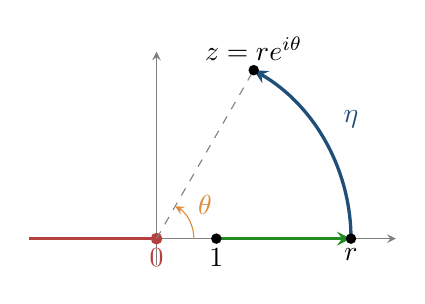
\begin{tikzpicture}[scale=0.95,>=stealth]
 \draw[gray,->] (-1.7,0)--(3.2,0);
 \draw[gray,->] (0,-0.35)--(0,2.5);
 \draw[exerciseframe,very thick] (-1.7,0)--(-0.06,0);
 \draw[fill=white,exerciseframe] (0,0) circle (2pt) node[below]{$0$};
 \draw[ForestGreen,very thick,->] (0.8,0)--(2.6,0);
 \draw[courseblue,very thick,->] (2.6,0) arc[start angle=0,end angle=60,radius=2.6];
 \draw[gray,dashed] (0,0)--(1.3,2.252);
 \draw[orangeframe,->] (0.5,0) arc[start angle=0,end angle=60,radius=0.5];
 \node[orangeframe] at (0.65,0.45){$\theta$};
 \fill (0.8,0) circle (2pt) node[below]{$1$};
 \fill (2.6,0) circle (2pt) node[below]{$r$};
 \fill (1.3,2.252) circle (2pt) node[above]{$z=re^{i\theta}$};
 \node[courseblue] at (2.6,1.6){$\eta$};
\end{tikzpicture}
\end{center}
On the real segment, the integral is $\int_1^r dx/x=\ln r$;
this also holds when $0<r<1$, with the segment traversed towards $r$.
Parametrize the arc by $\eta(u)=re^{iu\theta}$, $0\leq u\leq1$.
This parametrization works for either sign of $\theta$, and
\[
 \int_\eta\frac{d\zeta}{\zeta}
 =\int_0^1\frac{i\theta re^{iu\theta}}{re^{iu\theta}}\,du=i\theta.
\]
Therefore
\[
 \boxed{\Log z=\ln|z|+i\Arg z,\qquad -\pi<\Arg z<\pi.}
\]
The integral construction proves that this branch is holomorphic;
the polar formula evaluates it explicitly.

\begin{warning}
A branch does not satisfy $L(zw)=L(z)+L(w)$ without restrictions on the
arguments. For example, $z=w=e^{3\pi i/4}$ and $zw=-i$ all lie in $U_0$,
but
\[
 \Log(zw)=-\frac{\pi i}{2},\qquad \Log z+\Log w=\frac{3\pi i}{2}.
\]
The two sides differ by $2\pi i$.
\end{warning}

\end{document}
